\chapter{\IfLanguageName{dutch}{Stand van zaken}{State of the art}}%
\label{ch:stand-van-zaken}

% Tip: Begin elk hoofdstuk met een paragraaf inleiding die beschrijft hoe
% dit hoofdstuk past binnen het geheel van de bachelorproef. Geef in het
% bijzonder aan wat de link is met het vorige en volgende hoofdstuk.

% Pas na deze inleidende paragraaf komt de eerste sectiehoofding.

De huidige stand van zaken kan worden opgedeeld in 5 delen. Het eerste deel is een situatieschets van de huidige complete set-up van het \gls{dect}-systeem, met al zijn gebreken en voordelen. Deze voor- en nadelen worden dan verwerkt in het 2de deel. Hierin wordt er een oplijstinge gemaakt waaraan de nieuwe / vervangende technologieën aan moeten voldoen. Het overzicht is opgesteld via de MoSCoW techniek. Vervolgens is er een oplijsting van mogelijke alternatieven voor het \gls{dect}-systeemgevolgd door een uitdieping van de alternatieven hun eigenschappen en mogelijke gebruik. Om na de uiteenzetting afgetoetst te worden aan de requirements. Als voorlaatste deel wordt er gekeken naar de data en de implicatie hiervan. Dit hoofdstuk wordt afgesloten met een uiteenzetting van het huidige  securitylandschap.

\section{\IfLanguageName{dutch}{\gls{dect}-systeem}{\gls{dect}-system}}%
\label{sec:dect-systeem}
Het \gls{dect}-systeem staat voor Digital Enhanced Cordless Telecommunications; dit is een standaard in de EU sinds 1993. De meest gebruikte situatie is waar er meerdere gebruikers zijn voor een draadloze communicatie in werkomgevingen. De voornaamste reden voor gebruik van het \gls{dect}-draadloos systeem is dat het een grote dichtheid van veel gebruikers aankan \autocite{Welinder1997}. In vergelijking met andere mobiele communicatiesystemen werkt het niet buiten de werkomgeving \autocite{Welinder1997}. Na onderzoek van \textcite{Welinder1997} bleek dat de interferentie van het \gls{dect}-systeem op medisch gereedschap 11 procent was. De interferentie valt echter volledig weg bij een afstand van 0,5m tussen het gereedschap en het \gls{dect}-toestel.

%TODO: HOE DECT

Hoewel het \gls{dect}-systeem een standaard is sinds 1993, zijn er toch verschillende innovaties toegepast op dit systeem, maar deze worden als een apart systeem gezien. 
\\Het is belangrijk ook om te vermelden dat in deze bachelorproef enkel Intra-ziekenhuis communicatie wordt onderzocht. Dit betekent dat enkel binnen eenzelfde site wordt gekeken om een oplossing of alternatief te bieden voor het \gls{dect}-systeem.

Verder heeft het \gls{dect}-systeem volgens \textcite{Welinder1997}een hoge betrouwbaarheid, een groot bereik binnen gebouwen, lage energieconsumptie en een eigen frequentieband.
Deze frequenties liggen tussen 1880 MHz en 1900 MHz, opgesplitst in 10 kanalen. De kanalen opzich bestaan elk uit 12 duplex tijdsloten, dit resulteert in 120 bruikbare radiokanalen. \autocite{ETSI1999}

\section{\IfLanguageName{dutch}{Vereisten}{Requirements}}%
\label{sec:req}%



%---------

% Volgens \textcite{Coiera2006} zijn volgende aspecten van een communicatiesystemen voor ziekenhuizen van uiterst belang:

% \begin{enumerate}
%     \item Betrouwbaarheid en Beschikbaarheid
%     \item Beveiliging en Privacy
%     \item \acrfull{qos}
%     \item Interoperabiliteit
%     \item Mobilitetit en Dekking
%     \item Schaalbaarheid
%     \item Gebruiksvriendelijkheid
%     \item Integratie met (huidige) klinische workflows 
% \end{enumerate}

% Verder wordt er met het oog op de toekomst ook extra requirements toegevoegd. Deze zijn de volgende:

% \begin{enumerate}
%     \item Beschikbaarheid van Data
%     \item Prioritisering
% \end{enumerate}

% \textbf{DIT HOOFDSTUK ZAL WORDEN AANGEVULD TEGEN DE 2DE DEADLINE (SEMESTER 2)}

% \section{\IfLanguageName{dutch}{Betrouwbaarheid en Beschikbaarheid}{Reliability and Availability}}
% \label{sec:betrouwbaarheid-en-beschikbaarheid}
%


% \section{\IfLanguageName{dutch}{Beveiliging en Privacy}{Security and Privacy}}
% \label{sec:beveiliging-en-privacy}
%



% \section{\IfLanguageName{dutch}{Quality of Service}{Quality of Service}}
% \label{sec:quality-of-service}
%



% \section{\IfLanguageName{dutch}{Interoperabiliteit}{Interoperability}}
% \label{sec:interoperabiliteit}
% 



% \section{\IfLanguageName{dutch}{Mobilitetit en Dekking}{Mobility and Coverage}}
% \label{sec:mobilitetit-en-dekking}
% 



% \section{\IfLanguageName{dutch}{Schaalbaarheid}{Scalability}}
% \label{sec:schaalbaarheid}
% %



% \section{\IfLanguageName{dutch}{Gebruiksvriendelijkheid}{User-friendly Interface}}
% \label{sec:gebruiksvriendelijkheid}
%



% \section{\IfLanguageName{dutch}{Integratie met (huidige) klinische workflows}{Integration with Clinical Workflows}}
% \label{sec:integratie-met-klinische-workflows}
%
%---------
Voor de vereisten of requirements wordt er gebruik gemaakt van de MoSCoW techniek. Dit is een prioritisatie techniek uit het Agile framework. Volgens \textcite{2025agile} staan de letters voor:

\begin{itemize}
  \item \textbf{M}ust have - Noodzakelijk
  \item \textbf{S}hould have - Duidelijke meerwaarde
  \item \textbf{C}ould have - Niet-noodzakelijke meerwaarde
  \item \textbf{W}on't have this time - Niet in deze versie
\end{itemize}

Als er dan dieper wordt gekeken naar deze opdeling kan men bij elke categorie een verduidelijking plaatsen. Zo stelt \textcite{2025agile}:\\

\textbf{\textit{Must have}} bestaat uit de minimale oplijsting van vereisten die nodig zijn om het project te kunnen opleveren. Dit houdt in dat er gekeken wordt naar wetten, veiligheid, wat er als 'bare-minimum' moet zijn.\\

\textbf{\textit{Should have}} wordt beschreven als belangrijk maar niet noodzakelijk. Het project kan bestaan zonder, maar mogelijke workarounds zijn nodig alddanniet tijdelijk.\\

\textbf{\textit{Could have}} zijn zaken die een meerwaarde kunnen bieden, maar een minimale impact hebben indien niet geimplementeerd. Het verschil tussen should en could have ligt in de gradatie van problemen/pijn veroorzaakt indien er niet aan de vereiste wordt voldaan.\\

\textbf{\textit{Won't have}}, vereisten die op het eerste zich interessant zijn maar de laagste prioriteit krijgen. Dit is geen onderdeel van het huidige product/project, maar kan in de toekomst met een revisie worden geimplementeerd.\\

\subsection{Must have}
\label{sec:Must-have}

\begin{itemize}
  \item Wetgeving conform
  \subitem \gls{ehds}
  \subitem \gls{nis2}
  \subitem \gls{gdpr}
  \item Gesloten systeem
  \item Stabiel
  \item Communicatie-eisen
\end{itemize}

Volgens \textcite{Coiera2006} zijn de volgende zaken vereist om te spreken van een communicatiesysteem:
\begin{itemize}
  \item Communicatiekanaal
  \item Boodschap
  \item Communicatiebeleid
  \item Communicatietoestel
  \item Interacties
  \item Beveiligingsbeleid
\end{itemize}

\subsection{Should have}
\label{sec:Should-have}

\begin{itemize}
  \item Segregatie
  \item Opties voor meer dan enkel audiocommunicatie
\end{itemize}

\subsection{Could have}
\label{sec:Could-have}

\begin{itemize}
  \item Interne data gebruik mogelijk
  \item Monitoring software voor audits van het systeem
  \item AI controle systeem
\end{itemize}

\subsection{Won't have}
\label{sec:Wont-have}

\begin{itemize}
  \item Integratie medische apparatuur
  \item Monitoring software voor audits van het systeem
\end{itemize}

\section{\IfLanguageName{dutch}{Andere communicatietechnologieën}{Other communication Technologies}}%
\label{sec:andere}%

Op basis van studies van \textcite{Montalvo2024}, \textcite{Kranz2010} en \textcite{Soenmez2018} kan er een lijst worden opgesteld van alternatieven voor het \gls{dect}-systeem:

\begin{itemize}
  \item \gls{lte} Advanced
  \item 5G
  \item \gls{ule}
  \item \gls{voip}
\end{itemize}

Elke technologie wordt besproken op eenzelfde manier. Eerst wordt de techniek verklaard, vervolgens wordt de functionaliteit uitgeklaard. Eens deze duidelijk zijn wordt de technologie afgetoetst op de vereisten.

\subsection{\IfLanguageName{dutch}{\gls{lte} Advanced}{\gls{lte} Advanced}}%
\label{sec:ltea}%

\gls{lte} of Long Term Evolution is de overkoepelende technologie waaronder 5G valt. Volgens \textcite{Bakare2022} is ook een verbetering van \gls{lte} Advanced, een stap naar de toekomst van \gls{lte}. De voornaamste eigenschappen van \gls{lte} Advanced zijn, opgelijst door \textcite{Bakare2022}:

\begin{itemize}
  \item Drie keer beter in spectrumefficiëntie in vergelijking met \gls{lte}
  \subitem 30 bps/Hz downlink
  \subitem 15 bps/Hz uplink
  \item Datapiek 
  \subitem 1 Gbps downlink
  \subitem 500 Mbps uplink
  \item Ondersteuning voor schaalbare bandbreedte en spectrumaggregatie
  \item Lage latentie
  \item Zeer goede compatibiliteit met \gls{lte}
\end{itemize}

\subsection{\IfLanguageName{dutch}{5G}{5G}}%
\label{sec:5g}%
5G is een stap in de evolutie van het mobiele netwerk, opvolger van 4G. In deze bachelorproef gaat het om het private 5G-netwerk. Volgens \textcite{wen2021private} zijn er eigenschappen van private 5G die nauw aansluiten met die van \gls{dect}-systemen. De eerste eigenschap wijst op de hoge apparatuurdichtheid, maar bij 5G gaat deze ook nog eens gepaard met hoge throughput. Dit zorgt voor integratie van externe devices, zoals sensoren, camera's, etc. Vervolgens heeft 5G ook voordelen ten opzichte van \gls{dect}-systemen volgens \textcite{wen2021private}. Zo is er een hoge betrouwbaarheid met een lage latency. Deze lage latency geeft nieuwe mogelijkheden, zoals bv. een chirurgische ingreep vanop afstand.\\ De tweede eigenschap van het privaat netwerk is de flexibiliteit en voorspelbaarheid van \gls{qos}. Daarnaast zijn er verschillende architecturen die men kan implementeren om een privaat 5G-netwerk op te zetten. De eerste methode is een stand-alone deployment. Hierbij wordt een privaat netwerk opgezet, waarbij alle netwerk functies van het netwerk zijn gelimiteerd binnen een logische perimeter bestaande uit vooraf gedefinieerde regio's. De andere methode is een publiek netwerk geïntegreerd deployment. Deze architectuur kan worden opgesplitst in verschillende types, afhankelijk van de gradatie van integratie. Deze 4 types zijn de volgende:

\begin{itemize}
  \item \gls{o-ran}
  \item Gedeelde \gls{ran}
  \item Gedeelde \gls{ran} en controle vlak
  \item Gehost bij het Publieke Netwerk
\end{itemize}

\textcite{wen2021private} vermeldt ook dat er naast architectuur een keuze moet worden gemaakt voor het spectrum. Hier zijn ook opnieuw 3 keuzes: een dedicated privaat spectrum, een erkend spectrum en een niet-erkend spectrum. 
5G heeft een aantal noodzakelijke technologieën nodig in het netwerk. Een van deze technologieën is network slicing. Hierbij wordt er 'een netwerk in een netwerk' gemaakt door het fysieke netwerk op te splitsen in meerdere logische netwerken. Om aan network slicing te kunnen doen, is er een nood aan netwerkvirtualisatie. Het slicing zelf kan worden opgedeeld in 3 lagen: Infrastructuurlaag, Network-slice laag en Onderhoudslaag. De levensloop van het slicen van een netwerk verloopt volgens de volgende 4 fases \autocite{wen2021private}:

\begin{enumerate}
  \item Voorbereiding
  \item In dienst stellen
  \item Gebruik
  \item Ontmanteling
\end{enumerate}


\subsubsection{\IfLanguageName{dutch}{Publiek versus privaat}{Public versus private}}
\label{public-v-private}

Binnen België is het 5G spectrum door overheid vastgelegd. Volgens \textcite{Eede2023} zijn er 3 delen op het 5G spectrum:\\\\
Het eerste deel is een non-licensed deel, dit betekent dat dit vrij is voor iedereen. Dit deel ligt tussen de 2,40 en de 2,48 GHz. Op de deel van het 5G spectrum werkt onder andere WLAN, Bluetooth en ZigBee.\\
Het tweede deel wat wordt beheerd door de telecom providers.

\begin{table}[H]
\centering
\begin{tabular}{|l|l|l|}
\hline
\textbf{3600MHz-band}      & \textbf{Bandbreedte} & \textbf{Frequentiebereik}    \\ \hline
Citymesh Mobile NV         & 50 MHz               & 3430--3480 MHz               \\ \hline
PROXIMUS                   & 20 MHz               & 3580--3600 MHz               \\ \hline
Orange Belgium NV          & 100 MHz              & 3600--3700 MHz               \\ \hline
Proximus NV                & 100 MHz              & 3700--3800 MHz               \\ \hline
Telenet Group NV           & 100 MHz              & 3480--3580 MHz               \\ \hline
\end{tabular}
\caption{5G verdeling onder telecom providers. \autocite[Door][Copyright 2023 van]{Eede2023} \textcite{Eede2023}}
\end{table}


Tenslotte is er het laatste deel gereserveerd voor het 5G private netwerk.  Dit ligt tussen de 3,80 en de 4,20 GHz, wat betekend dat er 40 MHz beschikbaar is voor het private netwerk.


\subsubsection{\IfLanguageName{dutch}{Frameworks}{Frameworks}}
\label{framework}

Er zijn verschillende frameworks beschikbaar, maar met de focus op een toegankelijke methode zal er voornamelijk gefocust worden op open-source frameworks. Zo lijst \textcite{Eswaran2022} de verschillende variaties op een open-source 5G-framework voor private 5G-netwerken op:

\begin{itemize}
  \item Magma
  \item 5G OpenRAN
  \item ONF's Aether platform
  \item ETSI OSM
  \item \gls{srsRAN}
  \item OpenAirInterface \gls{ue}
\end{itemize}

Na verder onderzoek wordt ook \gls{open5gs} toegevoegd aan deze lijst.\\

Volgens \textcite{Open5GS2024} is Open5G 'een geavanceerd open-source project ontworpen voor het bouwen en onderhouden van je eigen NR/\gls{lte} mobiele netwerk. Open5G biedt een robuuste oplossing voor het configureren van zowel \gls{5gnr} als \gls{lte} (Evolved) netwerken.' \\ Verder zijn er andere concepten zoals \gls{o-ran}, waar onder andere het OpenCare5G-netwerk op gebaseerd is. In dit framework wordt Open RAN in een privaat netwerk gebruikt voor digitale gezondheidsapplicaties. Zo hebben \textcite{de2023opencare5g} onderzocht hoe dit framework kan gebruikt worden om gezondheidsonderzoeken te doen met draagbare ultrasone gereedschappen op verschillende locaties. Om deze onderzoeken te kunnen delen met artsen, werd er een lokaal privaat netwerk opgezet. Zo gebruikten ze een 5G xHaul ORAN \gls{oam} privaat netwerk. Er wordt gekozen om een top-down systeem te gebruiken. Dit is een georganiseerde manier om een netwerk project te ontwikkelen. Dit komt doordat men kan steunen op het OSI-model en het 5G-\gls{ran} protocol layer model. Dit zal ook gebruikt worden bij de methodologie. Zo zal er een analyse zijn van elke laag van de 5G-architectuur. Deze architectuur begint met de service laag. Op deze laag komen de verzoeken van de applicatie vandaan. De architectuur eindigt met de infrastructuurlaag. \autocite{de2023opencare5g}

\subsubsection{\IfLanguageName{dutch}{Simulatie}{Simulation}}
\label{sec:open5gs}

Alvorens er wordt gekeken naar \gls{open5gs}, moet er een opsplitsing worden gemaakt in de 5G realisatie.
Zo bestaan er volgens \textcite{Lee2025a} 2 type 5G-Cores:

\begin{itemize}
  \item 5G \gls{nsa} vereist een 4G topologie als backbone
  \item 5G \gls{sa}, is een systeem dat zonder andere netwerken kan werken.
\end{itemize}

Hieronder is een figuur die het hele 4G-/ 5G netwerk omvat. De reden dat 4G toch wordt vermeldt in dit schema, is omdat de de 5G \gls{nsa} topologie een 4G backbone nodig heeft. \autocite{Lee2025a}

\begin{figure}[H]
  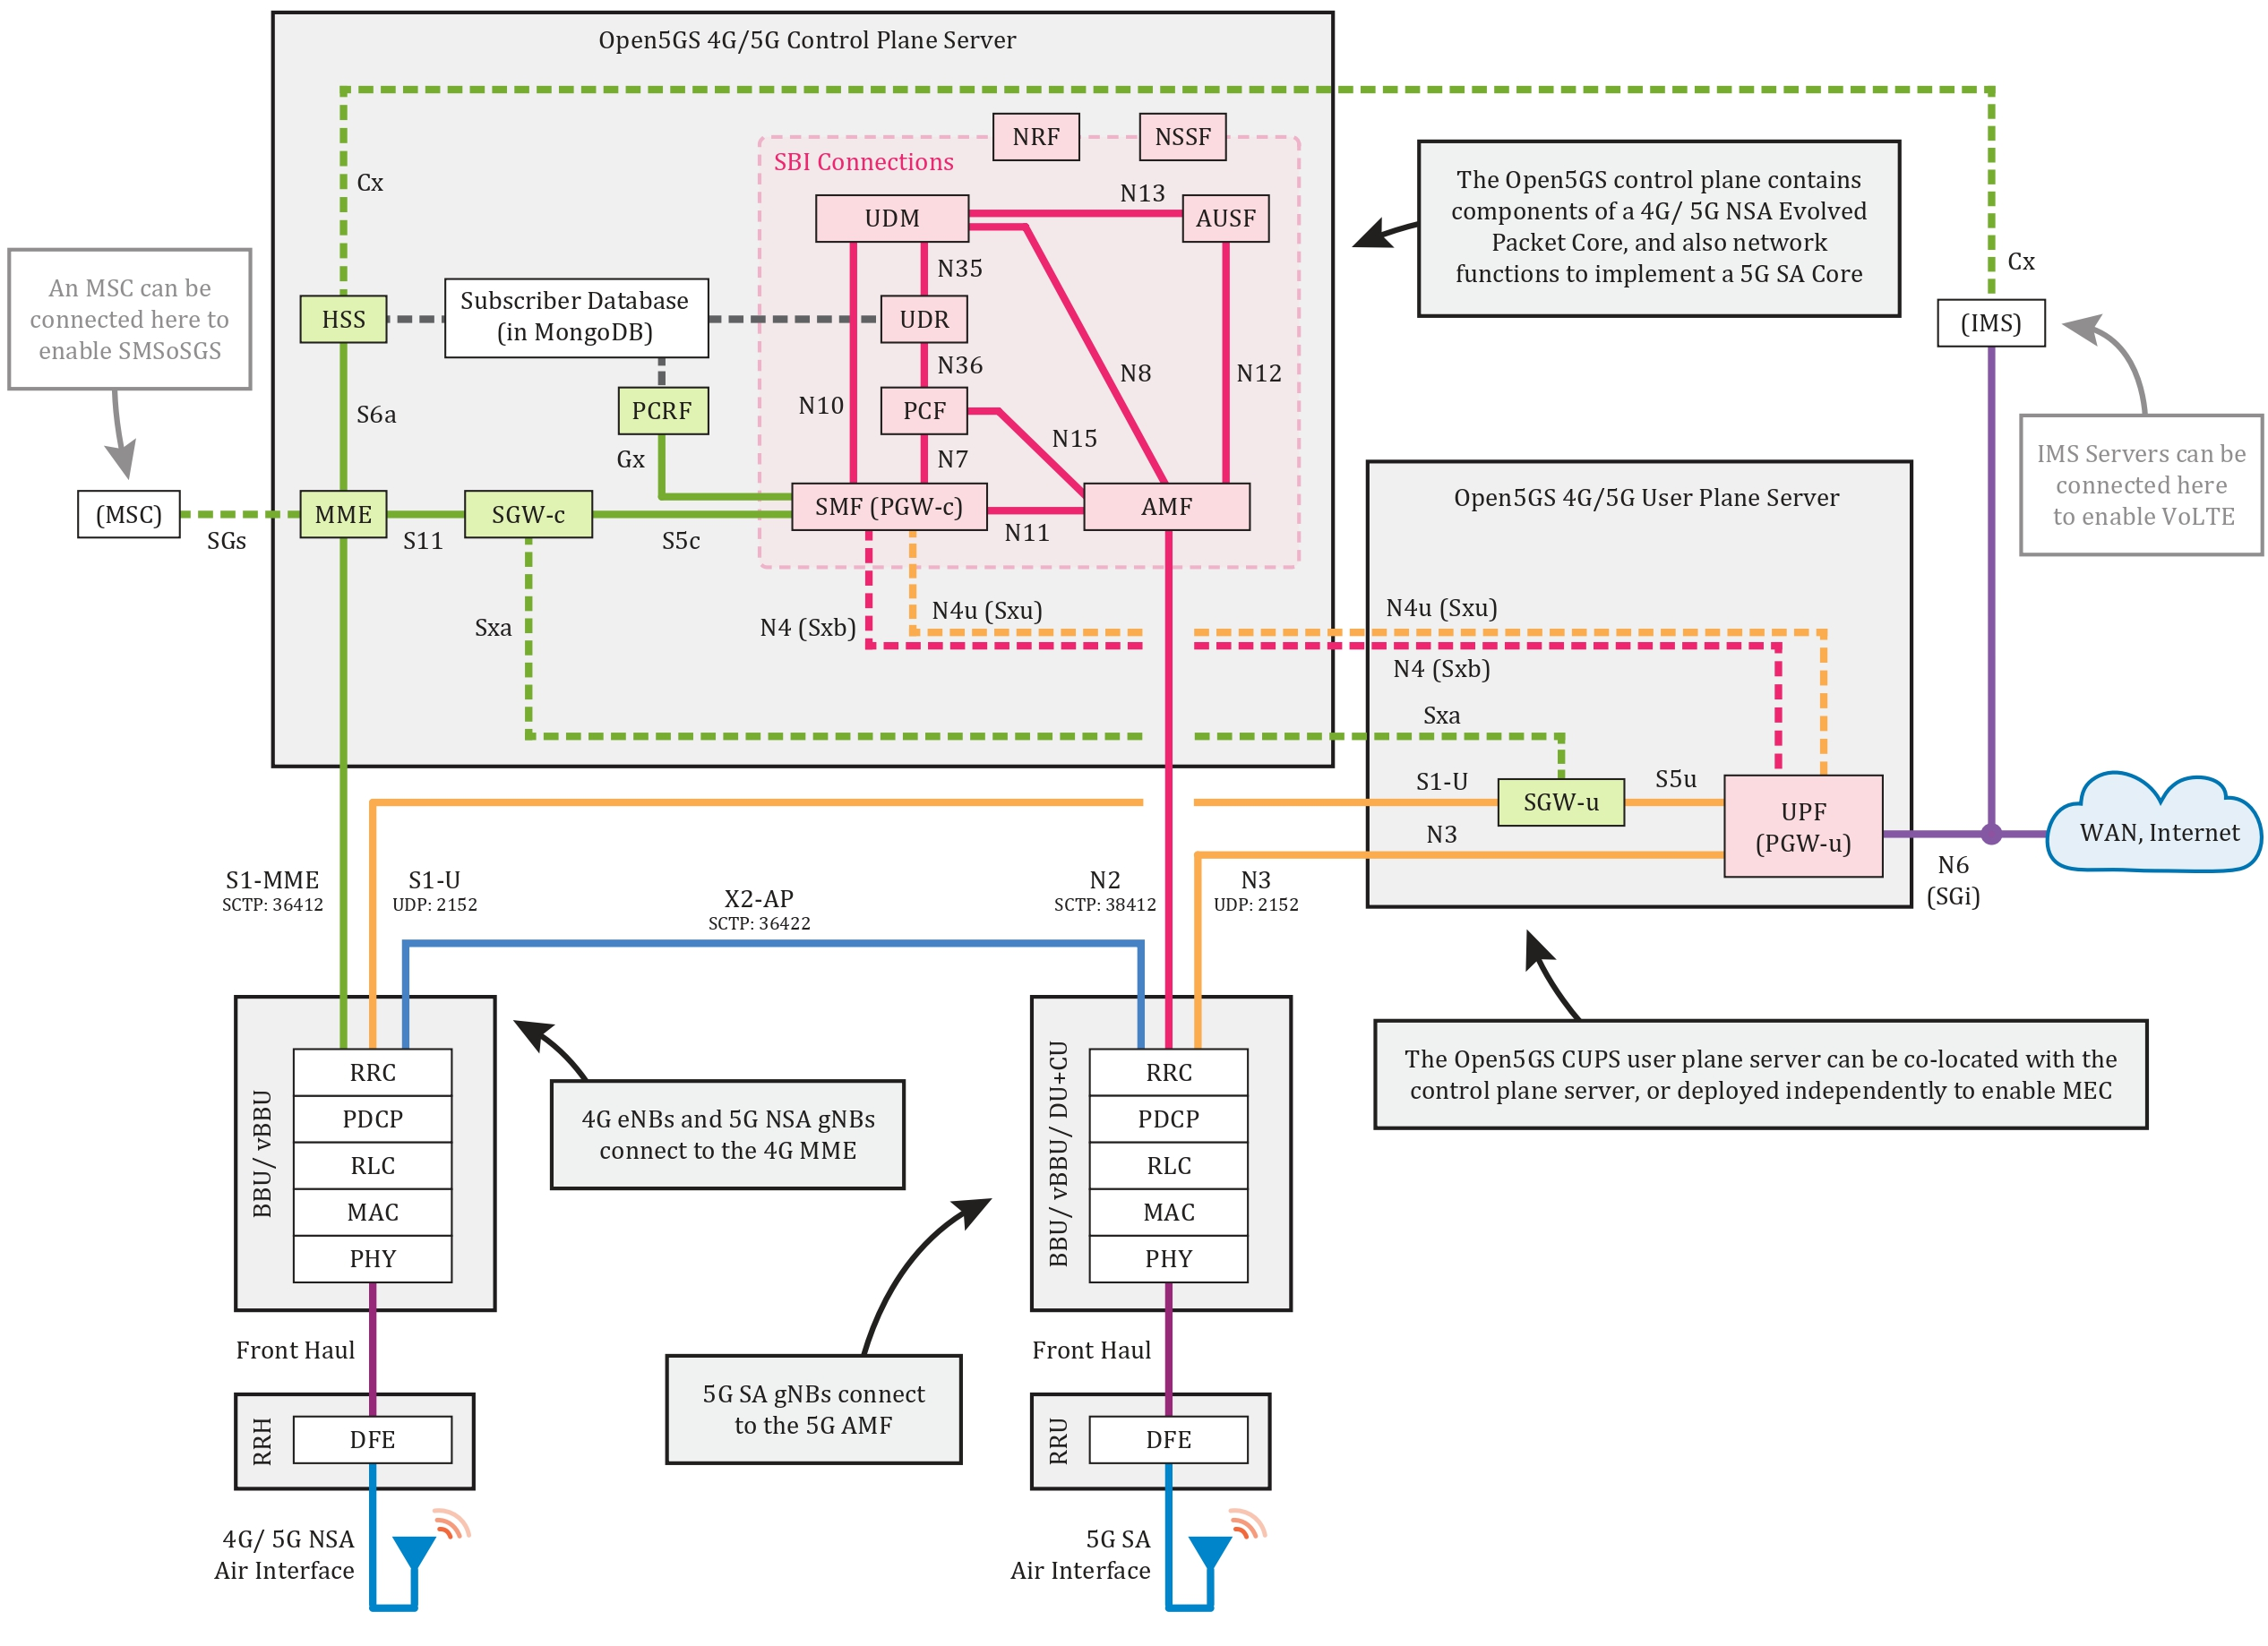
\includegraphics[width=\linewidth]{../graphics/Open5GS-Schema.jpg}
  \caption{Gesimuleerd 5G-netwerk met Open5GS. \autocite[Door][Copyright 2021 van]{Lee2021} \textcite{Lee2021}}
  \label{fig:open5gs-schema}
\end{figure}

\textbf{5G \gls{nsa} Core}\\\\
Volgens \textcite{Lee2025a} heeft de 5G \gls{nsa} Core volgende functies:

\begin{itemize}
  \item \gls{mme}
  \item \gls{hss}
  \item \gls{pcrf}
  \item \gls{sgwc}
  \item \gls{sgwu}
  \item \gls{pgwc-smf}
  \item \gls{pgwc-upf}
\end{itemize}

\textbf{5G \gls{sa} Core}\\\\

Volgens \textcite{Lee2025a} heeft de 5G \gls{nsa} Core volgende functies:

\begin{itemize}
  \item \gls{nrf}
  \item \gls{scp}
  \item \gls{sepp}
  \item \gls{amf}
  \item \gls{smf}
  \item \gls{upf}
  \item \gls{ausf}
  \item \gls{udm}
  \item \gls{udr}
  \item \gls{pcf}
  \item \gls{nssf}
  \item \gls{bsf}
\end{itemize}

Verder stelt \textcite{Lee2025a} ook dat 5G \gls{sa} gebruik maakt van een \gls{sba}. Dit betekent dat een duidelijke scheiding is tussen de Control Plan functies, geregistreerd in de \gls{nrf}, en de User Plane. Deze laatste bevat maar \'e\'en functie, namelijk de \gls{upf}.

Aangezien de simulatie via \gls{open5gs} wordt gedeployd en gekeken wordt vanuit een vervanging van het \gls{dect}-systeem, zal er geopteerd worden voor een 5G \gls{sa} Core. Om deze manier moet er niet eerst een 4G netwerk worden opgezet.

Verder zullen de \gls{gnb} en \gls{ue} worden gesimuleerd met \gls{ueransim}. Dit is ook een bijdragende factor voor de keuze voor de \gls{sa} opstelling, aangezien \gls{ueransim} enkel met dit type netwerken kan werken. Het is wel belangrijk om te vermelden dat \gls{ueransim} geen active ontwikkeling meer kent.

\subsubsection{\IfLanguageName{dutch}{Slicing}{Slicing}}
\label{sec:Slicing}

%TODO:

Shan2023

Foukas2017

\subsubsection{\IfLanguageName{dutch}{Kosten}{Costs}}
\label{sec:Cost}

Volgens \textcite{Abbas2024} is er een grotere kost dan enkel de aankoop van de installatie. Zo zijn er voor elke fase van het 5G installatie-project vaak verddoken kosten:

\begin{itemize}
  \item Planning kost
  \item Licensie kost 
  \item Infrastructuur kost (Hardware)
  \item Implementatie kost
  \item onderhoudskosten
  \item Use case kost (Opzetten van het project)
\end{itemize}

Zo verduidelijkt \textcite{Abbas2024} dat er in de implementatie fase al redelijk wat verdoken kosten zitten, zoals hieronder aangetoont.
\begin{figure}[H]
  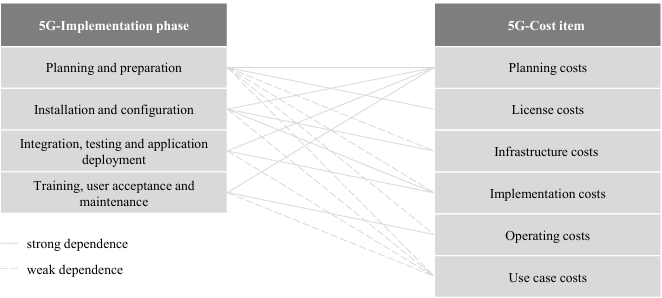
\includegraphics[width=\linewidth]{../graphics/kost-associaties.png}
  \caption{Afhankelijkheden tussen implementatie fase en kosten \autocite[Door][Copyright 2024 van]{Abbas2024} \textcite{Abbas2024}}
  \label{fig:Cost}
\end{figure}

Dit wordt ook aangetoond door \textcite{Hilary2024} dat men zich niet alleen mag focussen op de \gls{capex} van de 5G installatie, maar ook de \gls{opex}. Dit wordt nogmaals aangetoond doormiddel van de staafdiagrammen van \textcite{Hilary2024}

\begin{figure}[H]
  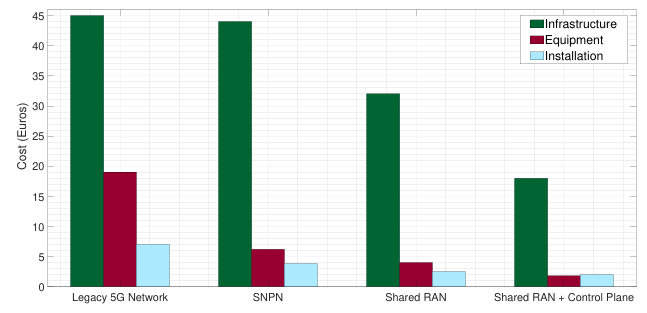
\includegraphics[width=\linewidth]{../graphics/capex.png}
  \caption{\gls{capex} van een 5G netwerk \autocite[Door][Copyright 2024 van]{Hilary2024} \textcite{Hilary2024}}
  \label{fig:capex}
\end{figure}

\begin{figure}[H]
  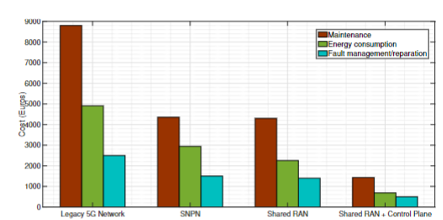
\includegraphics[width=\linewidth]{../graphics/opex.png}
  \caption{\gls{opex} van een 5G netwerk \autocite[Door][Copyright 2024 van]{Hilary2024} \textcite{Hilary2024}}
  \label{fig:opex}
\end{figure}

\begin{figure}[H]
  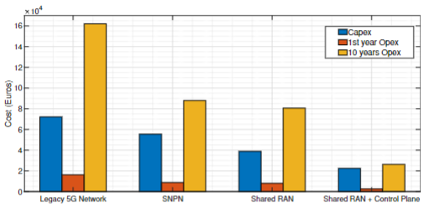
\includegraphics[width=\linewidth]{../graphics/capex-opex.png}
  \caption{Vergelijking van \gls{capex} met \gls{opex} op 1 jaar en op 10 jaar tijd \autocite[Door][Copyright 2024 van]{Hilary2024} \textcite{Hilary2024}}
  \label{fig:capex-vs-opex}
\end{figure}

\subsection{\IfLanguageName{dutch}{ULE}{ULE}}%
\label{sec:ule}%

\gls{ule} is een uitbreiding op het \gls{dect}-systeem zelf. Volgens \textcite{GariniDil2014} is dit een samenwerking tussen het \gls{dect}-systeem, \gls{cat-iq} (nieuwste HD voice-technologie) en een nieuwste aanpassing van data technologie \gls{ule} (Ultra Low Energy). Aangezien dit een uitbreiding is op het huidige \gls{dect}-systeem is er dus een makkelijke installatie en compatibiliteit.

De grootste voordelen van deze technologie volgens \textcite{GariniDil2014} zijn:

\begin{itemize}
  \item Open wereldwijde standaard
  \item Interferentievrije frequentieband
  \item Verbeterde veilige range
  \subitem Alle communicatie is versleuteld
  \item Lage kost
  \item Video en audio
\end{itemize}

%TODO: ULE uitleggen

Verder onderzoek door \textcite{Das2012} toont aan dat \gls{ule} ook een goede oplossing is voor de gezondheidszorg. Dit komt door de lage energieconsumptie, de lange levensduur van de batterij en de lage kosten. Dit maakt het een goede kandidaat voor een communicatiesysteem in de gezondheidszorg. Uit de deze studie (\textcite{Das2012}) kan men ook een oplijsting halen waarin verschillende technologieën worden vergeleken met het \gls{dect}-systeem. Dit is te zien in de tabel hieronder.

\begin{figure}[H]
  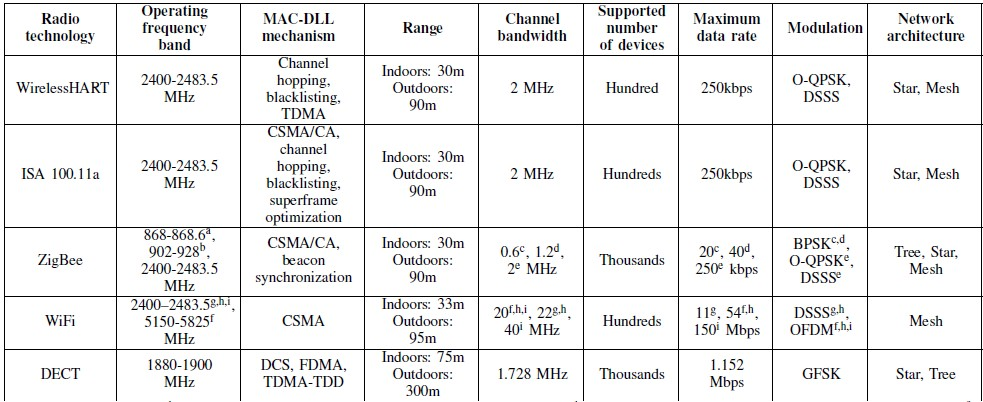
\includegraphics[width=\linewidth]{../graphics/overzicht.jpg}
  \caption{Overzicht \autocite[Door][Copyright 2012 van]{Das2012} \textcite{Das2012}}
  \label{fig:overzicht}
\end{figure}


Naast deze tabel, onderzocht \textcite{Das2012} kwaliteit van de channels die worden gebruikt door \gls{ule}. Verder wordt er naar de kans dat een channel selectie faalt in het \gls{ule}-systeem, de vertraging op communicatie en de gehele performantie vna het netwerk onder verschillende belastingen. Hieronder zijn een overzicht van de mogelijke channels die\gls{ule} kan gebruiken. Deze verschillende channels kan worden geïnterpreteerd als het \gls{ule} alternatief voor het 5G slicen.

\begin{figure}[H]
  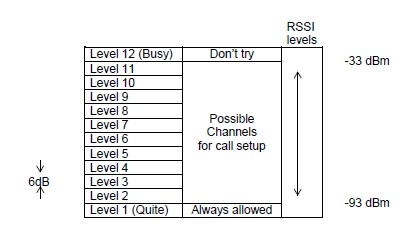
\includegraphics[width=\linewidth]{../graphics/ULE-channels.jpg}
  \caption{Lijst met channel selectie \autocite[Door][Copyright 2012 van \textcite{Das2012}]{Das2012}}
  \label{fig:ule-channels}
\end{figure}

\subsection{\IfLanguageName{dutch}{VoIP}{VoIP}}%
\label{sec:voip}%

\gls{voip} of Voice Communication over the Internet Protocol is een communicatietechnologie dat telefooncommunicatie stuurt over het internet in plaats van het telefoonnetwerk te gebruiken. \Autocite{Soenmez2018} Er zijn 5 scenario's waarin \gls{voip} kan worden gebruikt. Deze worden opgelijst door \textcite{Soenmez2018}:

\begin{itemize}
  \item Computer naar Computer
  \item Computer naar telefoon (\gls{pstn}) (of omgekeerd)
  \item Telefoon (\gls{pstn}) naar Telefoon (\gls{pstn})
  \item Mobiele \gls{voip}
  \item Draadloze \gls{voip}
\end{itemize}

Echter, \textcite{Soenmez2018} bevestigt wel dat er een groot aanvalsoppervlak bestaat. Zo heeft de \gls{voipsa} een lijst gepubliceerd met 6 beveiligingspunten waar countermeasures moeten geinstalleerd worden om een veilige omgeving te garanderen.

%TODO:
%TODO verklaar
\section{\IfLanguageName{dutch}{Data}{Data}}%
\label{sec:data}%

Volgens \textcite{Niekerk2020} is de gezondheidszorg rijk aan data en is deze data ook nog eens waardevol. Toch wordt er maar 50\% gebruikt.
De data kan een ondersteunende factor zijn om de alarmmoeheid weg te werken. Zo onderzocht \textcite{Hever2019} de mogelijkheid om met data en machine learning de valse alarmen te verminderen. In dat onderzoek werd dit getest op de Intensieve Zorg afdeling. In de conclusie van \textcite{Hever2019} stelt deze dat door het gebruik van deze data er een \gls{ai}-model opgeleid kon worden om de afdeling stiller en betrouwbaarder te maken. Dit verminderde het effect van alarmmoeheid. Verder meldt \textcite{Hever2019} dat door deze data en het model  ontbrekende factoren kunnen interpoleren.

\section{\IfLanguageName{dutch}{Beveiliging}{Security}}%
\label{sec:security}%

In samenspraak met de co-promotor is er geopteerd om cybersecurity niet actief te onderzoeken in deze bachelorproef. Echter, het is wel noodzakelijk om te weten dat er verschillende verplichtingen zijn in België en de Europese Unie. Als men een introductie van een 5G-netwerk uitvoert in een gezondheidszorgomgeving en/of ziekenhuizen is er sprake van een vergroting van de 'attack surface'. De beveiliging van dit type omgeving, ook wel de beveiliging van gezondheidszorg 5.0 genoemd, doet een beroep op de \gls{cia}-principes. Echter, \textcite{Wazid2022} voegt nog enkele extra eisen toe:

\begin{itemize}
  \item Beschikbaarheid
  \item Integriteit
  \item Vertrouwelijkheid
  \item Toegangscontrole
  \item Beschikbaarheid
  \item Voorwaartse geheimhouding
  \item Achterwaartse geheimhouding
  \item Onweerlegbaarheid
\end{itemize}

Als al deze principes worden toegepast, kan men stellen dat er voldaan is aan de minimum noodzakelijke beveiliging van het gezondheidszorgsysteem. Zo stelt \textcite{Wazid2022} vier reeds bestaande schema's voorop voor de beveiliging van dit systeem, elk met hun taak, features en beperkingen:

\begin{itemize}
  \item \gls{b2h} \autocite{Ghosh2022}
  \item Blockchain en quantum-blindhandtekening \autocite{Bhavin2021}
  \item Systeembreed sleutelschema \autocite{Chang2022}
  \item \gls{bits} \autocite{Gupta2020}
\end{itemize}
\subsection{\IfLanguageName{dutch}{Wetgevingen}{Laws}}%
\label{sec:wet}%

%TODO: Uitgebreider !!!

Sinds 27 april 2016 is de verordening 2016/679 van toepassing. Deze start de \gls{gdpr} (General Data Protection Regulation) in de Europese Unie. De verordening 2016/679 vermeldt dat "regels worden vastgelegd betreffende de bescherming van natuurlijke personen in verband met de verwerking van persoonsgegevens en het vrije verkeer van persoonsgegevens. Het beschermt de grondrechten en de fundamentele vrijheden van natuurlijke personen, met name hun recht op bescherming van persoonsgegeven."\\ (Verordening (EU) 2016/679 van het Europees Parlement en de Raad van 27 april 2016) %\autocite{gdpr2016} 
\\\\
Vervolgens is er ook het \gls{nis2}, een Belgische wet die bedrijven verplichtingen oplegt op het vlak van cybersecurity. "De wet van 26 april 2024 tot vaststelling van een kader voor de cyberbeveiliging van netwerk- en informatiesystemen van algemeen belang voor de openbare veiligheid (de "\gls{nis2}-wet") zet de EU-richtlijn 2022/2555 van het Europees Parlement en de Raad van 14 december 2022 (de "\gls{nis2}-richtlijn") om." \\
(Wet tot vaststelling van een kader voor de cyberbeveiliging van netwerk- en informatiesystemen van algemeen belang voor de openbare veiligheid van 26 april 2024) %\autocite{Belgium2024}
\\\\
Tenslotte is er een nieuwer initiatief genaamd \gls{ehds} (European Healthcare Data Space). Dit initiatief heeft het volgende doel: "De algemene doelstelling is te waarborgen dat natuurlijke personen in de EU in de praktijk meer zeggenschap over hun elektronische gezondheidsgegevens hebben."\\ (Voorstel (EU) COM/2022/197 van het Europees Parlement en de Raad van 3 mei 2022) %\autocite{\gls{ehds}2022}
